\section{Inovasi}
\label{sec:inovasi}

PowerShift adalah alat bantu keputusan berbasis web untuk merancang paket ``pensiun dini PLTU + PLTS atap'' di sistem Jawa-Bali. Alat ini menghitung siapa menanggung apa, yaitu PLN, APBN, dana luar, pelanggan, pekerja, dan warga di sekitar PLTU, setiap tahun dari 2026 sampai 2040. Gambar~\ref{fig:app} memperlihatkan tampilan utamanya.

\begin{figure}[H]
\centering
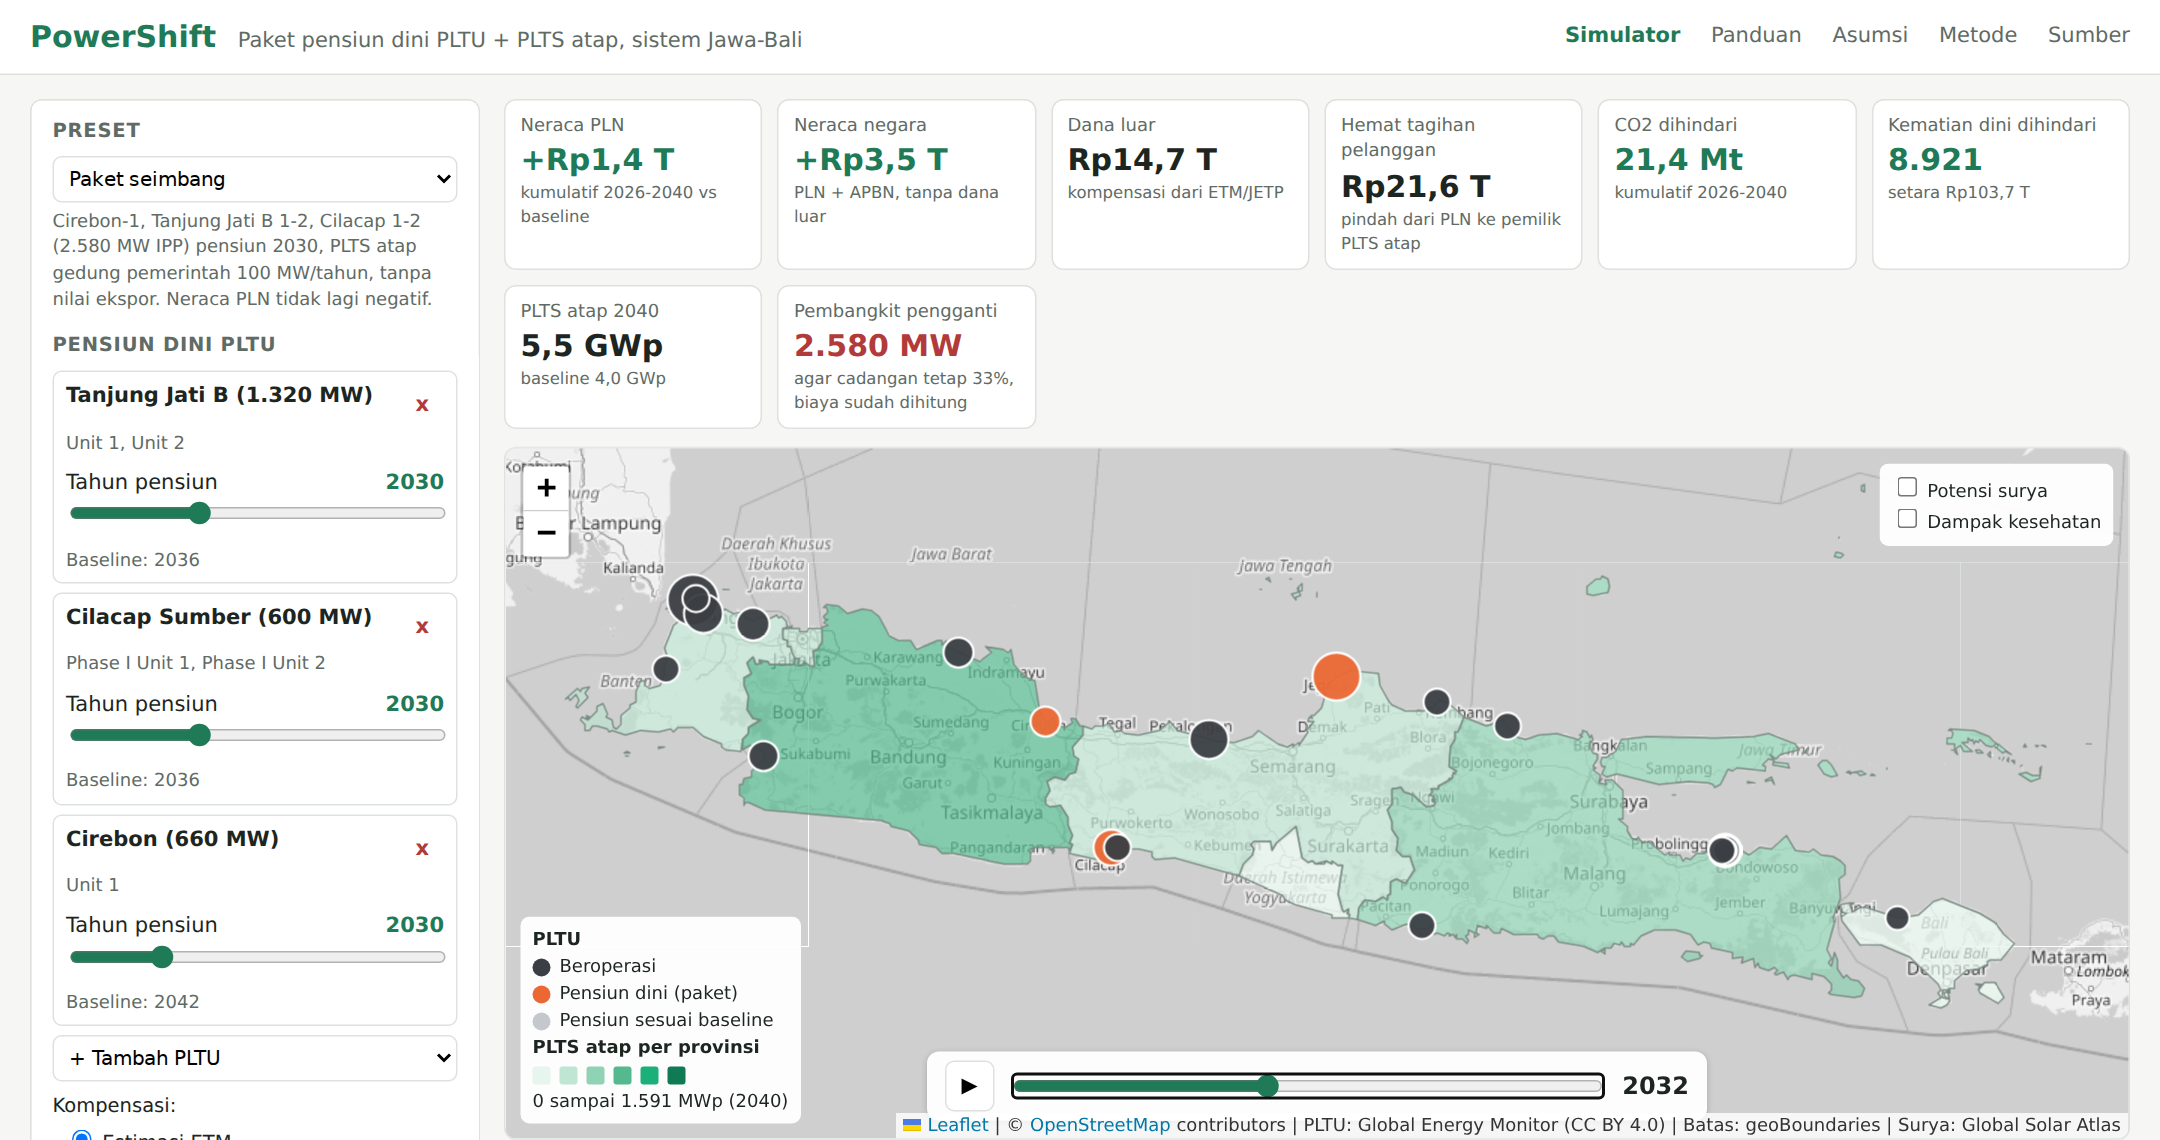
\includegraphics[width=\textwidth]{app_powershift}
\caption{Tampilan PowerShift untuk Paket seimbang pada tahun 2032. PLTU yang dipensiunkan dini berwarna jingga, warna provinsi menunjukkan kapasitas PLTS atap}
\label{fig:app}
\sumber{PowerShift, peta dasar OpenStreetMap contributors}
\end{figure}

\subsection{Kebaruan}

Alat yang sudah ada menjawab sebagian pertanyaan secara terpisah (Tabel~\ref{tab:kebaruan}). Belum ditemukan alat yang menghitung paket berpasangan PLTS atap terdistribusi dan pensiun PLTU per unit dari sisi neraca PLN dan APBN, padahal di titik inilah kebijakan selama ini macet.

\begin{table}[H]
\centering
\caption{PowerShift dibanding alat yang sudah ada}
\label{tab:kebaruan}
\small
\begin{tabularx}{\textwidth}{p{0.2\textwidth} X X}
\toprule
Alat & Yang dilakukan & Yang belum dilakukan \\
\midrule
Indonesia Energy Policy Simulator & Simulasi kebijakan nasional dan emisi \parencite{P-WRI-EPS} & Agregat nasional, tidak per PLTU dan tidak menghitung neraca PLN \\
TZ-CAT & Data per unit PLTU, biaya pengganti EBT skala besar \parencite{D-TZCAT,P-TZ-CONUNDRUM} & Lembar kerja untuk ahli, data 2022, tidak memuat PLTS atap \\
Kajian CREA dan IESR & Peringkat PLTU menurut biaya kesehatan \parencite{P-CREA-IESR-2023} & Laporan statis, tidak interaktif \\
SolarHub & Kalkulator PLTS atap per bangunan \parencite{P-SOLARHUB} & Tidak melihat dampak ke sistem dan PLN \\
En-ROADS & Simulator iklim global \parencite{P-ENROADS} & Tidak spesifik Indonesia \\
\midrule
PowerShift & Paket per unit PLTU dan PLTS atap, neraca PLN, APBN, dana luar, keandalan, kesehatan, kriteria Permen ESDM 10/2025, peta Jawa-Bali & Bukan model dispatch per jam \\
\bottomrule
\end{tabularx}
\sumber{penelusuran kelompok, November 2026}
\end{table}

\subsection{Cara Kerja}

Pengguna memilih PLTU dan tahun pensiunnya, nilai ekspor PLTS atap, kuota, PLTS atap gedung pemerintah, porsi subsidi yang dialihkan, sumber dana kompensasi, serta asumsi kompensasi (estimasi skema ETM atau klaim PLN). Model tahunan kemudian menghitung:
\begin{enumerate}
  \item \textbf{Adopsi PLTS atap.} Balik modal per segmen dihitung dari potensi surya per kabupaten \parencite{D-GSA-PVOUT}, tarif, dan porsi pemakaian sendiri. Perubahan adopsi mengikuti kurva pangsa pasar terhadap balik modal yang dipakai NREL \parencite{P-NREL-SOLARDS}, dibatasi kuota.
  \item \textbf{Neraca PLN.} Pendapatan yang hilang dan kompensasi ekspor dikurangkan, lalu ditambah biaya bahan bakar yang dihemat \parencite{B-KONTAN-DMO-2026}, pembayaran kapasitas IPP yang tidak lagi dibayar, dan dikurangi porsi kompensasi pensiun serta biaya pembangkit pengganti.
  \item \textbf{Neraca APBN dan negara.} Selisih PLN ditutup APBN, ditambah subsidi yang dihemat, tagihan gedung pemerintah yang dihemat, investasi PLTS pemerintah, dan porsi kompensasi APBN.
  \item \textbf{Keandalan.} Reserve margin dihitung dari data PLN dan MKI \parencite{B-MATAHARI-2024,B-PETROMINDO-RESERVE}. Mulai 2029 baseline dijaga di 33\%, sehingga PLTU yang pensiun dini harus diganti.
  \item \textbf{Dampak dan kriteria.} Emisi per unit dari GEM, kematian dini dari CREA, pekerja per MW, dan penilaian indikatif tujuh kriteria Pasal 11 Permen ESDM 10/2025.
\end{enumerate}

Hasil tampil sebagai kartu angka, peta PLTU dengan slider tahun 2026-2040, peta warna PLTS atap per provinsi, grafik neraca, dan tabel kriteria. Skenario dapat dibagikan lewat tautan, grafik serta data dapat diunduh, dan halaman Panduan menjelaskan setiap langkah penggunaan dengan tangkapan layar. PowerShift berupa situs statis (HTML, JavaScript, Leaflet, Chart.js) tanpa server sehingga dapat dihosting gratis \parencite{S-LEAFLET,S-CHARTJS}. Model diverifikasi dengan hitung tangan independen untuk Paket Cirebon-1 (Lampiran~\ref{app:hitung}) dengan selisih di bawah 0,01\%.

\subsection{Kecocokan untuk Indonesia}

PowerShift dibangun dari struktur yang khas Indonesia: PLN sebagai pembeli tunggal, kontrak take-or-pay IPP, harga batu bara DMO US\$70 per ton, subsidi 450/900 VA, oversupply Jawa-Bali yang akan habis, dan kriteria Permen ESDM 10/2025. Alat ini juga tidak membutuhkan data rahasia. Seluruh data berasal dari sumber terbuka (GEM, Global Solar Atlas, geoBoundaries), Statistik PLN \parencite{D-PLN-STAT-2025}, dan berita resmi, sedangkan parameter kontrak IPP yang tidak publik dapat diganti oleh pengguna yang memiliki data lebih baik, misalnya tim kajian PLN.
